\documentclass{article}
\usepackage[margin=1in]{geometry}
\usepackage{fancyvrb}
\usepackage{multicol}
\usepackage{hyperref}
\usepackage{amsmath}
\usepackage{amsfonts}

\usepackage[listings]{tcolorbox}

\definecolor{codegreen}{rgb}{0,0.6,0}
\definecolor{codegray}{rgb}{0.5,0.5,0.5}
\definecolor{codepurple}{rgb}{0.58,0,0.82}
\definecolor{backcolour}{rgb}{0.95,0.95,0.92}

\lstdefinestyle{mystyle}{
    language=Python,
    backgroundcolor=\color{backcolour},   
    commentstyle=\color{codegreen},
    keywordstyle=\color{magenta},
    numberstyle=\tiny\color{codegray},
    stringstyle=\color{codepurple},
    basicstyle=\ttfamily\footnotesize,
    breakatwhitespace=false,         
    breaklines=true,                 
    captionpos=b,                    
    keepspaces=true,                 
    numbers=left,                    
    numbersep=5pt,                  
    showspaces=false,                
    showstringspaces=false,
    showtabs=false,                  
    tabsize=2,
    escapechar=|,
    frame=single
}

\lstset{style=mystyle}

\newcommand{\showfig}[2]{
\noindent\includegraphics[width=\textwidth]{#1}
\centerline{#1}
}
\newcommand{\bi}{\begin{itemize}}
\newcommand{\li}{\item}
\newcommand{\ei}{\end{itemize}}

\usepackage{graphicx}
\usepackage{hyperref,fancyvrb,amsmath}
\usepackage{tikz}
\usepackage{tikz-qtree}

\newcommand{\mydot}[1]{\draw[fill] (#1) circle (0.1);}

\newcommand{\set}[1]{\ensuremath{\{#1\}}}

\title{Random Maze Generation}
\author{CSCI112, Lab 9}

\begin{document}

\maketitle
\centerline{\includegraphics[scale=1]{Figure_1}}

\begin{description}

\item[File names:]  Names of files, functions, and variables, 
when specified,
must be EXACTLY as specified.  This includes simple mistakes such
as capitalization.

\item[Individual work:]  All work must be your own.  Do not share
code with anyone other than the instructor and teaching assistants.
This includes looking over shoulders at screens with the code open.
You may discuss ideas, algorithms, approaches, {\em etc.} with
other students but NEVER actual code.  Do not use code
written by anyone else, in the class or from the internet.

\item[Documentation:] Each file should begin with a docstring
that includes your name, the class number and name, the lab
number, and  
a short description of the lab, as well as documentation pertinent
to that particular file.

  
\item[Maze algorithm:] To draw a maze, consider a rectangular grid
  with each cell labelled and walls between all adjacent cells. as in
  Figure \ref{mazefig} (a).  In the beginning, we regard each cell as
  in its own set by itself (since it is separated from the others by
  walls).  Thus, we have a {\em partition} of the set of $n$ cells
  into $n$ sets.  We will now gradually reduce the size of this
  partition to 1 by merging two sets at a time.

  We pick two adjacent cells from different sets at random, for
  example, 4 and 9.  We put a door (remove the wall) between them,
  merging their sets and getting Figure \ref{mazefig} (b), and we now
  have 24 sets of cells, all the sets not including 4 or 9, and the
  set \set{4,9}.

  We now pick another pair of adjacent cells at random, which are in
  {\em different} sets, for example 3 and 4, and put a door (remove a
  wall) between them.  This merges the sets \set{3} and the set
  \set{4,9} into the set \set{3,4,9}, and results in Figure
  \ref{mazefig} (c).


  Now we pick a different pair of random adjacent cells from different
  sets, for example 20 and 21, put a door between them and merge their
  sets, giving Figure
  \ref{mazefig} (d).


  We continue in this fashion, each time removing a wall between two
  random {\em adjacent} cells that are in {\em different} sets,
  merging the sets,  until
  we have only one set remaining, as in Figure \ref{mazefig} (e).  


At this point, we have a maze if we just remove the cell labels
and leave an entrance at the upper left, and an
exit at the lower right, as in Figure \ref{mazefig} (f).
  
It is crucial that we always pick a pair of adjacent cells from {\em
  different} sets.  If they are not adjacent putting a door between
them makes no sense.  If they are in the same partition, our maze
would have cycles in it.


\item[Picking random adjacent cells:] As the algorithm progresses,
  there will be fewer and fewer adjacent cells in different
  partitions.  If we just pick cells at random, it will take longer
  and longer to find a candidate to merge.  To solve this we take the
  following approach.

  Before we begin, we form a complete list of all adjacent cell pairs.
  Each cell in the grid is paired up with the cells to
  the right and below it, if they exist.  For example, for the cells
  in Figure \ref{mazefig}, the list would start out looking like this:
  \[
  ((0,1), (0,5), (1,2), (1,6), (2,3), (2,7), (3,4), (3,8), (4,9),
  (5,10), \ldots, (21,22), (22,23), (23,24) )
  \]
  Note that some cells (on the right side and the bottom) have only
  one adjacent cell, and the last cell has no adjacent cell.

  Now we randomize this list.  The algorithm is simple:  for each
  pair of cells, swap that pair with a pair at a random location.  Or
  you can use the {\tt random.shuffle} routine.

  We use this list every time we want a new pair of random cells.  We
  remove the first pair and check to see if the two cells are in
  different partitions.  If they are in different partitions, we put a
  door there and merge the partitions.  We also eliminate
  this pair from our list of walls.  If we don't put a door there (they were
  in the same partition), we keep them in the {\tt walls} list.

  We can now use the resulting list of remaining {\tt walls} to tell us where all the
  internal walls are drawn in the final maze.  Having this list makes
  it easy to draw the final maze: draw the outside border (leaving the
  entrance and exit open), and then draw a wall segment between each
  pair of cells in the {\tt walls} list.

\item[Merging  and detecting disjoint sets:]
  
Now that we have a random pair of cells, another problem is maintaining
the partition of the cells, with the following operations as fast as
possible: 
  \begin{itemize}
  \item Determine if two cells are in the same partition.
    \item Merge two partitions into one.
  \end{itemize}

If we do this inefficiently, every time we have two cells, $i$ and
$j$, and want to know if they are in the same set, we may have to use
an $O(n)$ process to find this out.  We can do a lot better than that.

For these trees we are only going to use {\em parent} pointers, and
they will be general trees, not binary trees.  Rather than create a 
data structure for the cells with a parent pointer, we'll use a 
dictionary of parents, with the keys being the cells.

Each cell starts out in its own tree, as in Figure \ref{mergesets}
(a).   Thus, each cell has {\tt None} as its parent.
   
In order to merge cells 4 and 9, we simply make the root of
one the parent of the root of the other; for example as in Figure
\ref{mergesets} (b), where we made 9 the parent of 4.  In (c) we
join 3 and 4 by merging \set{3} with \set{4,9}, by making 9 the
parent of 3 (since 9 is the root of \set{4,9}).  The next few merges
are shown in Figure \ref{mergesets} (d) to (h).  (Which cells were
merged at each step?)

Clearly, given two cells, merging their sets is a fast operation.  We
merely find their roots, and then make the root of one be the parent
of the other.

But what about determining if two nodes are in the same partition?

The beauty here is that it is going to be very fast to find the root
of each cell's tree.  Two cells are in the same set if they have the
same root.  For example, in Figure \ref{mergesets} (h), cells 3 and 20
are in different sets, because $\mbox{root}(3) = 19 \not =
21 = \mbox{root}(20) $.




\end{description}

\begin{figure}
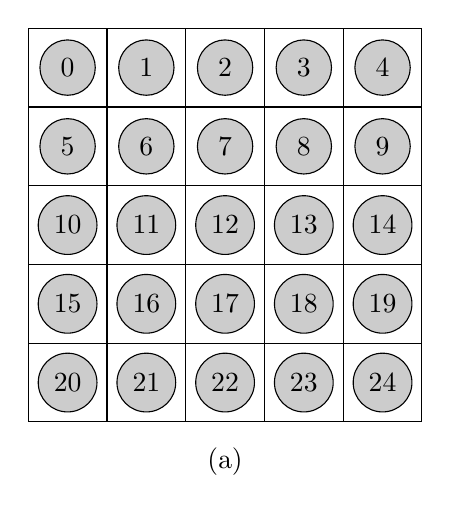
\begin{tikzpicture}[scale=1.0,darkstyle/.style={circle,draw,fill=gray!40,minimum size=20}]
  \foreach \x in {0,...,4}
    \foreach \y in {0,...,4} 
       {\pgfmathtruncatemacro{\label}{\x - 5 *  \y +20}
       \node [darkstyle]  (\x\y) at (0.5+\x,0.5+\y) {\label};} 

 \draw (5,0) -- (5,5) -- (0,5);
  \foreach \x in {0,...,4}
    \foreach \y in {0,...,4}
      \draw (\x, \y) -- (1+\x, \y)
            (\x, \y) -- (\x, 1+\y)
      ;
 \draw  (2.5,-0.5) node {(a)};
\end{tikzpicture}\hfill
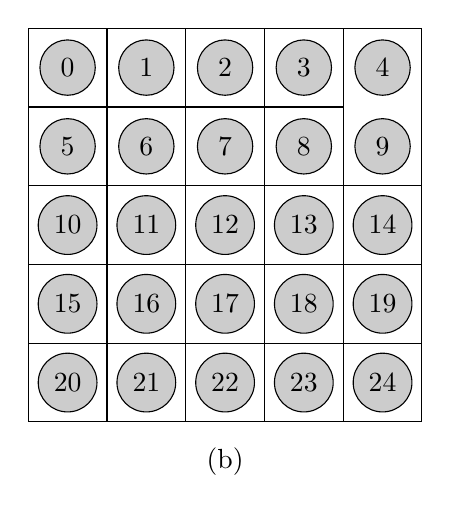
\begin{tikzpicture}[scale=1.0,darkstyle/.style={circle,draw,fill=gray!40,minimum size=20}]
  \foreach \x in {0,...,4}
    \foreach \y in {0,...,4} 
       {\pgfmathtruncatemacro{\label}{\x - 5 *  \y +20}
       \node [darkstyle]  (\x\y) at (0.5+\x,0.5+\y) {\label};} 

 \draw (5,0) -- (5,5) -- (0,5) -- (0,0) -- cycle;
  \foreach \x in {0,...,4}
    \foreach \y in {0,...,3}
      \draw (\x, \y) -- (1+\x, \y)
            (\x, \y) -- (\x, 1+\y)
      ;
    \foreach \x in {0,...,4}
       \draw (\x,4) -- (\x,5);
    \foreach \x in {0,...,3}
       \draw (\x,4) -- (1+\x,4);
 \draw  (2.5,-0.5) node {(b)};
\end{tikzpicture}\hfill
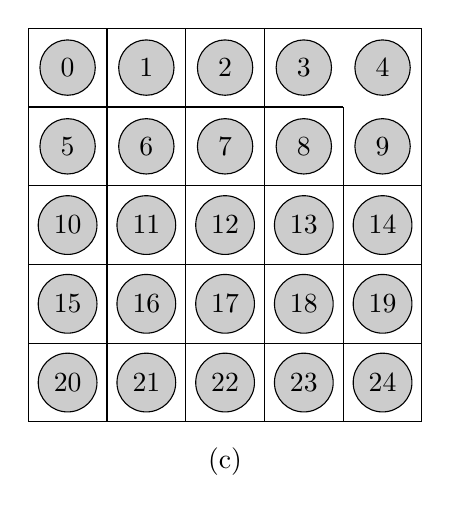
\begin{tikzpicture}[scale=1.0,darkstyle/.style={circle,draw,fill=gray!40,minimum size=20}]
  \foreach \x in {0,...,4}
    \foreach \y in {0,...,4} 
       {\pgfmathtruncatemacro{\label}{\x - 5 *  \y +20}
       \node [darkstyle]  (\x\y) at (0.5+\x,0.5+\y) {\label};} 

 \draw (5,0) -- (5,5) -- (0,5) -- (0,0) -- cycle;
  \foreach \x in {0,...,4}
    \foreach \y in {0,...,3}
      \draw (\x, \y) -- (1+\x, \y)
            (\x, \y) -- (\x, 1+\y)
      ;
    \foreach \x in {0,...,3}
       \draw (\x,4) -- (\x,5);
    \foreach \x in {0,...,3}
       \draw (\x,4) -- (1+\x,4);
 \draw  (2.5,-0.5) node {(c)};
\end{tikzpicture}

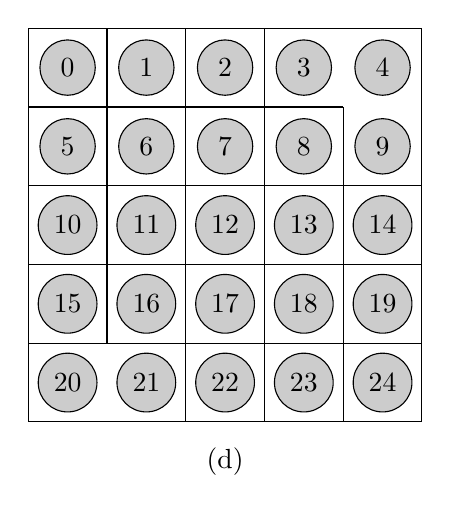
\begin{tikzpicture}[scale=1.0,darkstyle/.style={circle,draw,fill=gray!40,minimum size=20}]
  \foreach \x in {0,...,4}
    \foreach \y in {0,...,4} 
       {\pgfmathtruncatemacro{\label}{\x - 5 *  \y +20}
       \node [darkstyle]  (\x\y) at (0.5+\x,0.5+\y) {\label};} 

 \draw (5,0) -- (5,5) -- (0,5) -- (0,0) -- cycle;
  \foreach \x in {0,...,4}
    \foreach \y in {1,...,3}
      \draw (\x, \y) -- (1+\x, \y)
            (\x, \y) -- (\x, 1+\y)
      ;
    \foreach \x in {0,...,3}
       \draw (\x,4) -- (\x,5);
    \foreach \x in {0,...,3}
    \draw (\x,4) -- (1+\x,4);
    \foreach \x in {2,...,4}
    \draw (\x,0) -- (\x,1);
 \draw  (2.5,-0.5) node {(d)};
\end{tikzpicture}\hfill
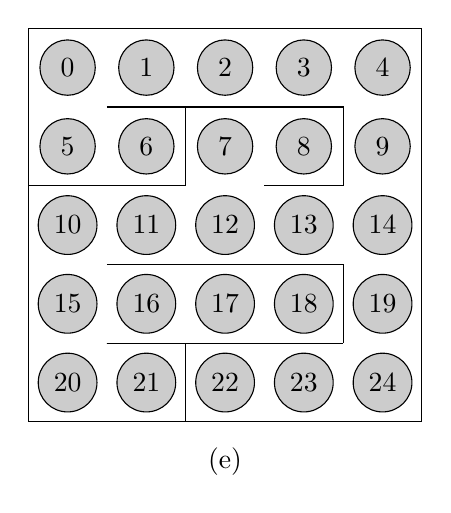
\begin{tikzpicture}[scale=1.0,darkstyle/.style={circle,draw,fill=gray!40,minimum size=20}]
  \foreach \x in {0,...,4}
    \foreach \y in {0,...,4} 
       {\pgfmathtruncatemacro{\label}{\x - 5 *  \y +20}
       \node [darkstyle]  (\x\y) at (0.5+\x,0.5+\y) {\label};} 

 \draw (5,0) -- (5,5) -- (0,5) -- (0,0) -- cycle;
 \draw (2,0) -- (2,1) -- (1,1) -- (2,1) -- (3,1) -- (4,1)
       (1,2) -- (2,2) -- (3,2) -- (4,2) -- (4,1)
       (0,3) -- (1,3) -- (2,3) -- (2,4) -- (1,4)
       (1,4) -- (2,4) -- (3,4) -- (4,4) -- (4,3) -- (3,3)
 ;
 \draw  (2.5,-0.5) node {(e)};
\end{tikzpicture}\hfill
\begin{tikzpicture}[scale=1.0,darkstyle/.style={circle,draw,fill=gray!40,minimum size=20}]

 \draw (1,5) -- (5,5) -- (5,0) (4,0) -- (0,0) -- (0,5);
 \draw (2,0) -- (2,1) -- (1,1) -- (2,1) -- (3,1) -- (4,1)
       (1,2) -- (2,2) -- (3,2) -- (4,2) -- (4,1)
       (0,3) -- (1,3) -- (2,3) -- (2,4) -- (1,4)
       (1,4) -- (2,4) -- (3,4) -- (4,4) -- (4,3) -- (3,3)
 ;
 \draw  (2.5,-0.5) node {(f)};
\end{tikzpicture}
\caption{Merging cells to make a maze.  The original partition is (a),
after merging \set{4} and \set{9} we get (b), after merging \set{3}
and \set{4,9} we get (c), and after merging \set{20} and \set{21} we
get (d).  A full merge down to one set is shown in (e), and drawn as a
maze in (f).}
\label{mazefig}
\end{figure}


  \begin{figure}

(a)  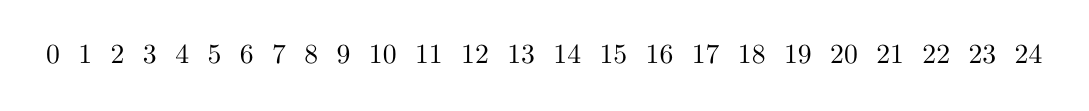
\begin{tikzpicture}
    \matrix {
  \Tree [.0 ] &
  \Tree [.1 ] &
  \Tree [.2 ] &
  \Tree [.3 ] &
  \Tree [.4 ] &
  \Tree [.5 ] &
  \Tree [.6 ] &
  \Tree [.7 ] &
  \Tree [.8 ] &
  \Tree [.9 ] &
  \Tree [.10 ] &
  \Tree [.11 ] &
  \Tree [.12 ] &
  \Tree [.13 ] &
  \Tree [.14 ] &
  \Tree [.15 ] &
  \Tree [.16 ] &
  \Tree [.17 ] &
  \Tree [.18 ] &
  \Tree [.19 ] &
  \Tree [.20 ] &
  \Tree [.21 ] &
  \Tree [.22 ] &
  \Tree [.23 ] &
  \Tree [.24 ] \\
};
\end{tikzpicture}

      \hrulefill
      
(b)  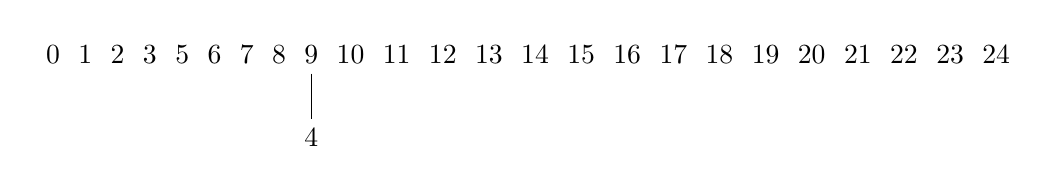
\begin{tikzpicture}
    \matrix {
  \Tree [.0 ] &
  \Tree [.1 ] &
  \Tree [.2 ] &
  \Tree [.3 ] &
  \Tree [.5 ] &
  \Tree [.6 ] &
  \Tree [.7 ] &
  \Tree [.8 ] &
\Tree [.9  [.4 ] ] &
  \Tree [.10 ] &
  \Tree [.11 ] &
  \Tree [.12 ] &
  \Tree [.13 ] &
  \Tree [.14 ] &
  \Tree [.15 ] &
  \Tree [.16 ] &
  \Tree [.17 ] &
  \Tree [.18 ] &
  \Tree [.19 ] &
  \Tree [.20 ] &
  \Tree [.21 ] &
  \Tree [.22 ] &
  \Tree [.23 ] &
  \Tree [.24 ] \\
};
\end{tikzpicture}

      \hrulefill
      

(c)  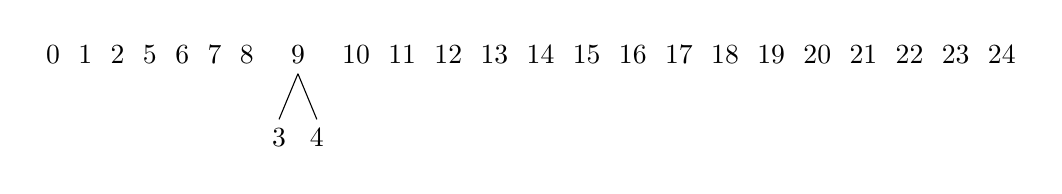
\begin{tikzpicture}
    \matrix {
  \Tree [.0 ] &
  \Tree [.1 ] &
  \Tree [.2 ] &
  \Tree [.5 ] &
  \Tree [.6 ] &
  \Tree [.7 ] &
  \Tree [.8 ] &
\Tree [.9  [.3 ] [.4 ] ] &
  \Tree [.10 ] &
  \Tree [.11 ] &
  \Tree [.12 ] &
  \Tree [.13 ] &
  \Tree [.14 ] &
  \Tree [.15 ] &
  \Tree [.16 ] &
  \Tree [.17 ] &
  \Tree [.18 ] &
  \Tree [.19 ] &
  \Tree [.20 ] &
  \Tree [.21 ] &
  \Tree [.22 ] &
  \Tree [.23 ] &
  \Tree [.24 ] \\
};
\end{tikzpicture}


      \hrulefill
      


(d)  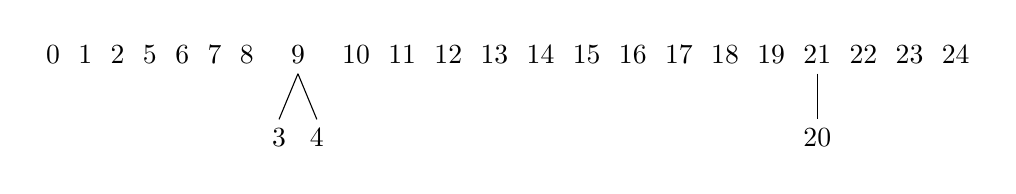
\begin{tikzpicture}
    \matrix {
  \Tree [.0 ] &
  \Tree [.1 ] &
  \Tree [.2 ] &
  \Tree [.5 ] &
  \Tree [.6 ] &
  \Tree [.7 ] &
  \Tree [.8 ] &
\Tree [.9  [.3 ] [.4 ] ] &
  \Tree [.10 ] &
  \Tree [.11 ] &
  \Tree [.12 ] &
  \Tree [.13 ] &
  \Tree [.14 ] &
  \Tree [.15 ] &
  \Tree [.16 ] &
  \Tree [.17 ] &
  \Tree [.18 ] &
  \Tree [.19 ] &
  \Tree [.21 [.20 ] ] &
  \Tree [.22 ] &
  \Tree [.23 ] &
  \Tree [.24 ] \\
    };
  \end{tikzpicture}

      \hrulefill
      


(e)  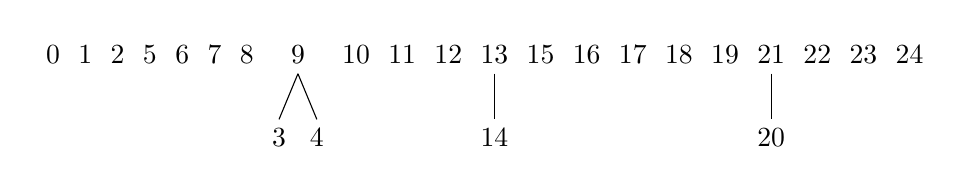
\begin{tikzpicture}
    \matrix {
  \Tree [.0 ] &
  \Tree [.1 ] &
  \Tree [.2 ] &
  \Tree [.5 ] &
  \Tree [.6 ] &
  \Tree [.7 ] &
  \Tree [.8 ] &
\Tree [.9  [.3 ] [.4 ] ] &
  \Tree [.10 ] &
  \Tree [.11 ] &
  \Tree [.12 ] &
  \Tree [.13 [.14 ] ] &
  \Tree [.15 ] &
  \Tree [.16 ] &
  \Tree [.17 ] &
  \Tree [.18 ] &
  \Tree [.19 ] &
  \Tree [.21 [.20 ] ] &
  \Tree [.22 ] &
  \Tree [.23 ] &
  \Tree [.24 ] \\
    };
  \end{tikzpicture}


      \hrulefill
      

(f)  \begin{tikzpicture}
    \matrix {
  \Tree [.0 ] &
  \Tree [.1 ] &
  \Tree [.2 ] &
  \Tree [.5 ] &
  \Tree [.6 ] &
  \Tree [.7 ] &
  \Tree [.8 ] &
\Tree [.9  [.3 ] [.4 ] [.13 [.14 ] ] ] &
  \Tree [.10 ] &
  \Tree [.11 ] &
  \Tree [.12 ] &
  \Tree [.15 ] &
  \Tree [.16 ] &
  \Tree [.17 ] &
  \Tree [.18 ] &
  \Tree [.19 ] &
  \Tree [.21 [.20 ] ] &
  \Tree [.22 ] &
  \Tree [.23 ] &
  \Tree [.24 ] \\
    };
  \end{tikzpicture}


      \hrulefill
      


(g)  \begin{tikzpicture}
    \matrix {
  \Tree [.0 ] &
  \Tree [.1 ] &
  \Tree [.2 ] &
  \Tree [.5 ] &
  \Tree [.6 ] &
  \Tree [.7 ] &
  \Tree [.8 ] &
  \Tree [.10 ] &
  \Tree [.11 ] &
  \Tree [.12 ] &
  \Tree [.15 ] &
  \Tree [.16 ] &
  \Tree [.17 ] &
  \Tree [.18 ] &
  \Tree [.19 [.9  [.3 ] [.4 ] [.13 [.14 ] ] ]   ] &
  \Tree [.21 [.20 ] ] &
  \Tree [.22 ] &
  \Tree [.23 ] &
  \Tree [.24 ] \\
    };
  \end{tikzpicture}
  
 \hrulefill
      
(h)  \begin{tikzpicture}
    \matrix {
  \Tree [.0 ] &
  \Tree [.1 ] &
  \Tree [.2 ] &
  \Tree [.5 ] &
  \Tree [.6 ] &
  \Tree [.7 ] &
  \Tree [.8 ] &
  \Tree [.10 ] &
  \Tree [.11 ] &
  \Tree [.12 ] &
  \Tree [.15 ] &
  \Tree [.16 ] &
  \Tree [.17 ] &
  \Tree [.18 ] &
  \Tree [.19 [.9  [.3 ] [.4 ] [.13 [.14 ] ] ] [.24 ]  ] &
  \Tree [.21 [.20 ] ] &
  \Tree [.22 ] &
  \Tree [.23 ] \\
    };
  \end{tikzpicture}



  \caption{Merging sets with trees.  Which two cells are merged at
    each stage? }
  \label{mergesets}
  \end{figure}
  
 \begin{description}
 \item[Implementation:]
  
  We can implement these ideas with just two major data structures:
  {\tt walls} and {\tt parents}.  
  
  \begin{description}
  \item[{\tt parents}] is a dictionary with each cell in the maze being
  a key, and the value is either {\tt None} or another
  cell in the maze.  This is initialized to all {\tt None},
  indicating that each cell is alone in its own class.
  
  \item[{\tt walls}] is a list of {\em pairs} of cells, indicating that there is a wall
  between the two cells.  To begin with, there is a wall between
  every adjacent pair of cells in the maze.  
  
  Since we only need to represent
  a wall once, we don't need to store both the north and south walls,
  for example, or both the east and west walls.  We arbitrarily 
  decide that each cell will hold only the south and east neighbors
  (as in the algorithm discussion, above).
  
  Make sure that the cells along the edges do not have
  neighbors that are off the board!
  
 \end{description}
 
 With these data structures it is easy to implement the functions
 we need.
 \begin{itemize}
 \item {\tt root}: find the root of a cell from the {\tt parents}
 \item {\tt join}: join the two sets of cells in different sets into one set
 \item  {\tt eraseWalls:} loop through the list of walls and eliminate
 them one by one as we unify cells, in line with the above algorithm
 \item {\tt drawMaze} one simple way to draw a set of lines is with
 {\tt matplotlib}.  Import the plotting object with
 \begin{lstlisting}
import matplotlib.pyplot as plt
\end{lstlisting}
Here is my code:
\begin{lstlisting}
def drawMaze(walls, mazeSize):
    nrows, ncols = mazeSize
    fig,ax = plt.subplots()
    ax.axis('off')
    plt.plot((0,ncols,ncols),
             (nrows,nrows,1),
             linestyle='-',color='black')
    plt.plot((ncols,0,0),
             (0,0,nrows-1),
             linestyle='-',color='black')
    for wall in walls:
        i,j = wall
        y1,x1 = position(i,mazeSize)
        y2,x2 = position(j,mazeSize)
        if x1 == x2:
            plt.plot((x1, x1+1), (y1,y1), linestyle='-',color='black')
        else:
            plt.plot((x1,x1), (y1,y1+1), linestyle='-',color='black')    
    plt.show()
\end{lstlisting}
In my implementation I represented cells as single integers, as in
the notes above, hence I needed to translate an integer into
a two dimensional position with the {\tt position} function.
If you represent cells as pairs, you may not need this step.
\end{itemize}

\item[Analysis:]  Note that the whole algorithm is $O(n\log n)$,
where $n$ is the number of cells.  There are about $2n$ walls,
and for each wall we check whether the endpoints are in
the same class with about $\log n$ steps, thanks to the forest of trees.
If we have to join two sets, it is a $O(1)$ process, again thanks
to the forest of trees.
Without this optimization, it is very easy for these kinds of
algorithms to become $O(n^2)$ or worse.
\end{description}
\end{document}
